\documentclass[11pt, a4paper]{article}

\usepackage{amsmath}
\usepackage{amsfonts} %Matheschriften
\usepackage{amssymb} %Mathesymbole
%\usepackage{mathptmx} % Einstellung für Schriften und Sonderzeichen in mathematischen Umgebungen
                        % ändert SChriftfont
\usepackage{wasysym} % Stellt diverse Sonderzeichen bereit
\usepackage{siunitx}
\usepackage{float}
\usepackage{microtype}
\usepackage{graphicx}
\usepackage{hyperref}
\usepackage{xcolor}
\usepackage[section]{placeins}
% allows for temporary adjustment of side margins
\usepackage{changepage}
\usepackage{rotating}


\usepackage[ngerman]{babel}
\addto\captionsngerman{%
 \renewcommand{\abstractname}{Einleitung}}

\title{Versuch 2: Interferometer}
\author{Team 4-11: Jascha Fricker, Benedict Brouwer}

\begin{document}
    \maketitle

    \tableofcontents

    \newpage

    \section{Einleitung}

    Interferometer werden im der Messtechnik für viele verschiedene Aufgaben benutzt. Das Micherlson-Interferometer ist eines der bekanntesten Arten von Interferometer, welches unter anderem beim Michelson-Morley Experiment zum Bestimmung der Äther-Geschwindigkeit benutzt wurde. In diesem Versuch benutzen wir es um den Brechungsindex von Plexiglas und Luft zu bestimmen.

    \section{Theorie}
    \subsection{Ganghöhenbestimmung}

    Mithilfe der Formeln
    \begin{align}
        \Delta s = \frac{N \cdot \lambda}{2}
    \end{align}4
    kann man die Verschiebung des Spiegels $\Delta s$ durch die Anzahl der Maxima $N$ und berechnen. Für die Ganghöhe wollen wir den Abstand pro Einheit
    \begin{align}
        g = \frac{\Delta s}{\Delta x} = \frac{N \lambda}{2 \Delta x}
    \end{align}
    haben, wobei $x$ Anzahl der Umdrehungen ist. 

    \subsection{Brechungsindex Luft}
    Mit folgenden Formeln sind Brechungindex $n$, Druck $p$ und Anzahl gezählter Maxima $N$ verknüpft
    \begin{align}
        N \cdot \lambda &= 2 l \cdot \Delta n \\
        n = 1 + \frac{\chi}{T} p \label{eq:luft} \\ 
        N \cdot \lambda &= 2 l \cdot \frac{\chi}{T} \Delta p
    \end{align}
    wobei $l$ die Länge der evakuierbaren Kammer ist.

    \subsection{Brechungsindex Plexiglas}
    Durch Drehung der Plexiglsscheibe mit Dicke $d$ um Winkel $\alpha$ kann der Brechungsindex $n$ bestimmt werden.
    \begin{align}
        N \cdot \lambda &= 2 \cdot h \cdot \left(1 - n - cos(\alpha) + \sqrt{n^2 - sin^2(\alpha)}\right) \\
        tan(\alpha) &= \frac{x + c}{d}
    \end{align}
    wobei $N$ die Anzahl an Maxima $x$ die Länge der Schraube und $d$ der Abstand der Schraube vom Drehpunkt ist.

    \section{Ergebnisse}
    \subsection{Ganghöhe}

    Aus den gemessenen Daten lässt sich eine Ganghöhe des Spiegels von
    \begin{align}
        g = 19.03(9) \si{\nano\metre}
    \end{align}
    pro Einheit Schraubendrehung bestimmen. Als Fehler wurden wegen der analogen Messung eine Ungenauigkeit von $0.21$ Einheiten angenommen.  
    
    \subsection{Brechungsindex Luft}

    Durch einen Fit der Formel \ref{eq:luft}, wie im Graphen \ref{fig:druck} gezeigt, kann die Proprtionalitätskonstante
    \begin{align}
        \chi = 7,52(11) \cdot 10^{-10} \si{\kelvin\per\pascal}
    \end{align}
    zwiscchen Druck und Brechungsindex bestimmt werden. Berücksichtigt wurden Unsicherheiten beim Luftdruck und bei der Temperatur.

    \begin{figure}
        \centering
        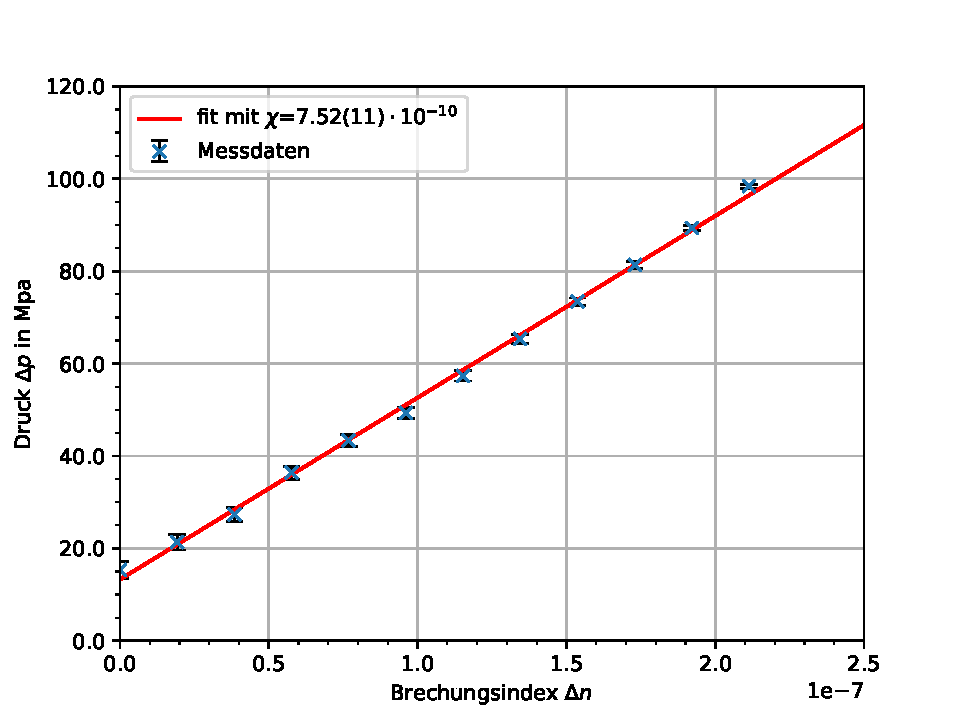
\includegraphics[width=0.8\textwidth]{./plots/druck.pdf}
        \caption{Druckabhängigkeit Brechungindex}
        \label{fig:luft}
    \end{figure}

    \section{Diskussion}

    \bibliographystyle{plain}
    \bibliography{literature}

\end{document}